\section{АЛГОРИТМІЧНЕ ЗАБЕЗПЕЧЕННЯ ПРОЦЕСУ СТВОРЕННЯ КОРПОРАТИВНОЇ СИСТЕМИ}

\subsection{Загальні вимоги до програмного продукту}
Основою будь-якої корпоративної системи є можливість можливість використання системи управління користувачами.
Тому слід розробити повний цикл взаємодії користувачів. Сюди повинні бути включені наступні такі важливі аспекти:
\begin{enumerate}
	\item можливість авторизації користувачів;
	\item ролі користувачів;
	\item зберігання даних у закодованому вигляді;
	\item чіткий розподіл прав користувачів;
	\item легка взаємодія між користувачами;
	\item можливість інтеграції із іншими сервісами системи.
\end{enumerate}

\par Тому слід розглянути кожний пункт більш детально.

\subsubsection{Авторизація користувачів}
Кожний працівник (він же користувач системи) повинний мати безперебійний доступ до свого профілю в будь-який час.  


\subsection{Проектування системи}
На початку розробки будь-якого програмного продукту слід значну увагу приділити проектування системи, адже саме від цього буде залежати легкість і правильність подальшої розробки системи, її підтримка і удосконалення.
Саме тому проектування визначає основну складову програмного забезпечення. 
Необхідні пункти для успішного запуску  продукту:
\begin{enumerate}
	\item побудова UML діаграми класів;
	\item побудова діаграми відношень між об'єктами;
	\item проектування бази даних;
	\item створення макетів майбутнього інтерфейсу;
	\item чітке розмежування модулів системи і їх взаємодія і тому подібне.
\end{enumerate}

\par Як було згадано вище, перш за все слід розробити діаграму класів, показати всі взаємовідношення між об'єктами, їх роль у системі та загальну взаємодію.
\subsubsection{Проектування UML діаграми класів}


TODO
Короче щось тут сказати про проектування, а то бошка щось не варить)))
В залежності від того, як буде спроектовано систему в цілому, буде
Додати архітектуру сайту
всякі технології опис, і буде купа сторінок:)
\subsection{Структура проекту}

\subsubsection{Проектування бази даних}
Як і кожний великий проект, даний проект повинний працювати із базою даних.

\begin{center}
		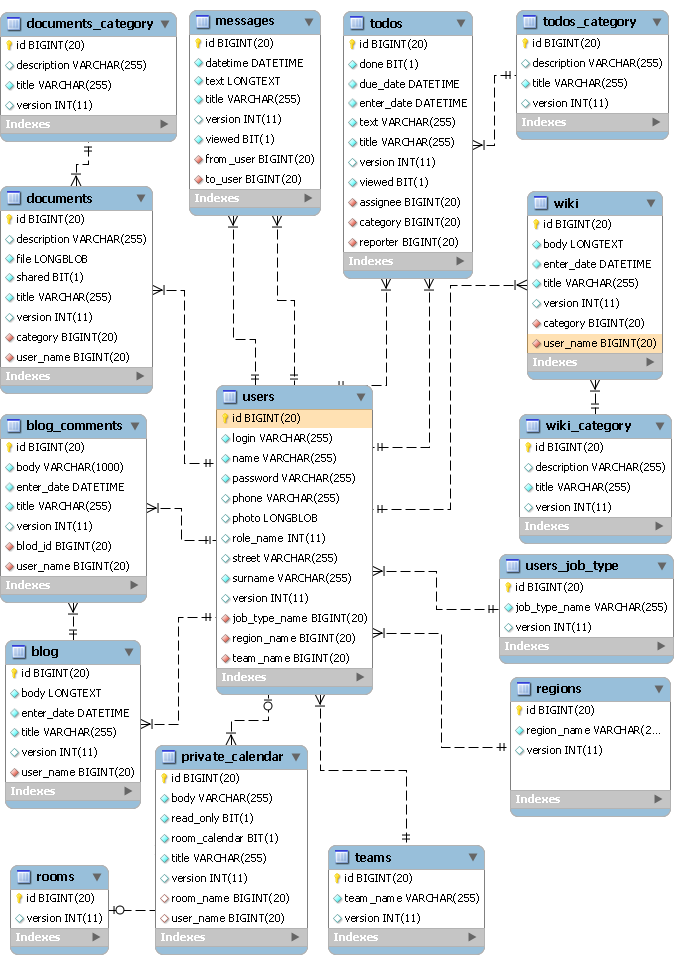
\includegraphics[width=1.00\textwidth]{db_schema.png}
		\captionof{figure}{Загальна схема структури бази даних}
\end{center}


\begin{center}
		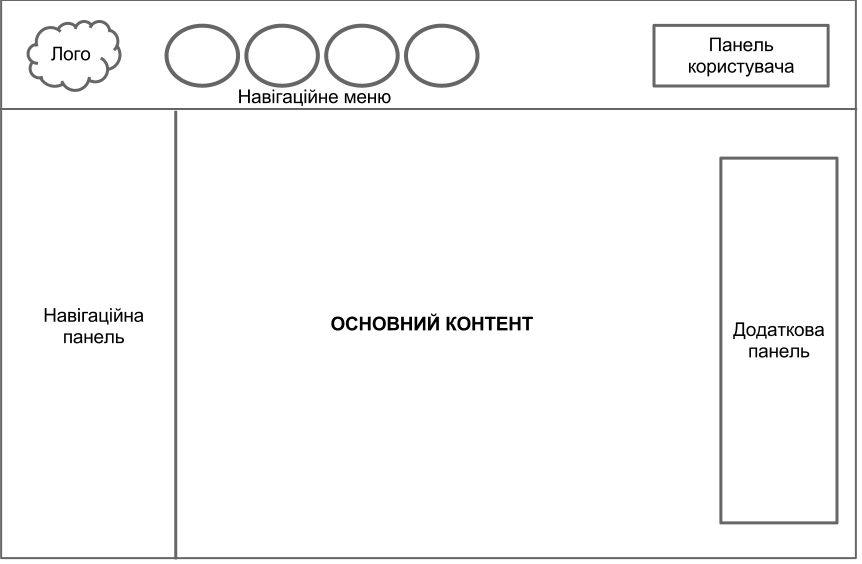
\includegraphics[width=1.00\textwidth]{mockup_mainpage.png}
		\captionof{figure}{Макет майбутнього сайту}
\end{center}


\begin{center}
		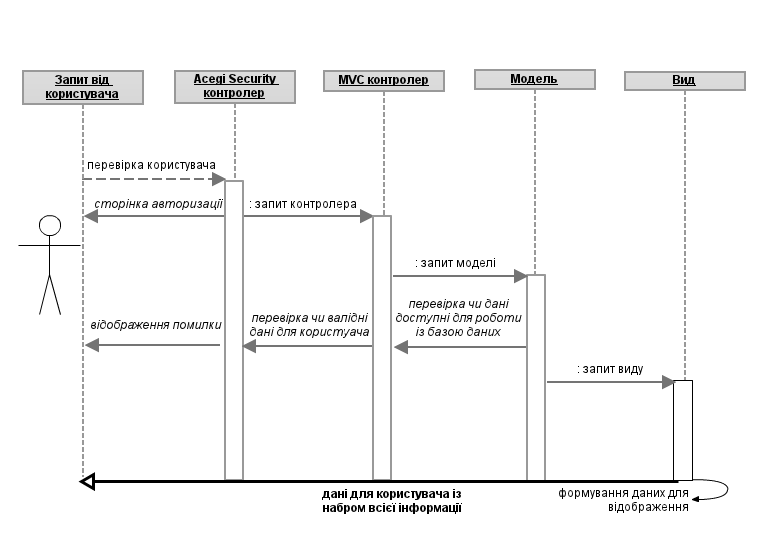
\includegraphics[width=1.00\textwidth]{sequence_diagram.png}
		\captionof{figure}{Діаграма відношення запиту користувача до роботи сервера}
\end{center}
